\documentclass[11pt]{article}

\newcommand{\HWnum}{4} 
\newcommand{\StudName}{Timothy Holmes} % author
\newcommand{\CourseNum}{474}           % course number
\newcommand{\Subject}{PHY}

\usepackage{graphicx, amsmath, amssymb,fancyhdr}
\addtolength{\textwidth}{1.5in}
\addtolength{\oddsidemargin}{-2cm}
\addtolength{\evensidemargin}{-2cm}
\addtolength{\textheight}{1.6in}
\addtolength{\topmargin}{-0.7in}
\addtolength{\headsep}{-0.1in}
%\addtolength{\footskip}{-0.2in}
\pagestyle{fancy}
\cfoot{}
\lhead{\textbf{\Subject ~ \CourseNum~--- Homework~\HWnum}}
\rhead{\textbf{\StudName:~Page~\thepage}}

\addtolength{\parskip}{\baselineskip} % skips a line between paragraphs
\parindent 0in                        % no indent at start of paragraph

\newcommand{\dd}{\textrm{d}}
\usepackage{braket}
\usepackage{lipsum, babel}
\usepackage{blindtext}
\usepackage{graphicx}% Include figure files
\usepackage{dcolumn}% Align table columns on decimal point
\usepackage{bm}% bold math
\usepackage{listings}
\usepackage{listing}
\usepackage{supertabular}



\usepackage{color} %red, green, blue, yellow, cyan, magenta, black, white
\definecolor{mygreen}{RGB}{28,172,0} % color values Red, Green, Blue
\definecolor{mylilas}{RGB}{170,55,241}



\lstset{language=Python,%
    %basicstyle=\color{red},
    breaklines=true,%
    morekeywords={matlab2tikz},
    keywordstyle=\color{blue},%
    morekeywords=[2]{1}, keywordstyle=[2]{\color{black}},
    identifierstyle=\color{black},%
    stringstyle=\color{mylilas},
    commentstyle=\color{mygreen},%
    showstringspaces=false,%without this there will be a symbol in the places where there is a space
    numbers=left,%
    numberstyle={\tiny \color{black}},% size of the numbers
    numbersep=9pt, % this defines how far the numbers are from the text
    emph=[1]{for,end,break},emphstyle=[1]\color{red}, %some words to emphasise
    %emph=[2]{word1,word2}, emphstyle=[2]{style},    
}

\begin{document}
% -------------------------- BOD -------------------------- 

\title{Homework {\HWnum}}
\author{Timothy Holmes \\ \Subject ~ \CourseNum ~ Stellar Astrophysics}

\maketitle

\section*{Problem 1}
Consider the PP-I chain that we learned in class. Calculate the energy released in each of the three steps of the PP-I chain, express your answer in MeV.

The PP-I chain is made up of the following reactions:

(To get from units of $u$ to $MeV$ we can use the equation $\Delta E = (u) \cdot (kg/u) \cdot c^{2} = J$, then we can convert $J = 6.24 \times 10^{12} MeV/J$.) 

\begin{align*}
&{}^{1}H + {}^{1}H = {}^{2}H + e^{+} + \nu \\
&2 * (7.28 \; MeV) \rightarrow 13.14 MeV + 0.51 \; MeV + 0 \; MeV = 0.42 \; MeV\\ \\
&{}^{2}H + {}^{1}H = {}^{3}He + \gamma \\
&13.14 \; MeV + 7.29 \; MeV \rightarrow 14.93 \; MeV + 0 \; MeV = 5.49 \; MeV\\ \\
&{}^{3}He + {}^{3}He = {}^{4}He + 2{}^{1}H  \\
&2 * (14.93 \; MeV)\rightarrow 2.42 \; MeV + 2 * (7.29 \; MeV) = 11.29 \; MeV\\
\end{align*}



\clearpage

\section*{Problem 2}

Nuclear fusion converts H to He, so the mass fractions X and Y are going to change from the beginning of the Main Sequence (ZAMS) to the end of the Main Sequence (also known as TAMS). In this problem, you will calculate X and Y at TAMS.

\subsubsection*{(a)}

The Sun's luminosity is in units of Watts, therefore, this value is the energy value. Using 

$$
E = mc^{2}
$$

to find how much mass is lost every second we can rewrite the equation as

$$
m = \frac{E}{c^{2}} = \frac{3.838 \times 10^{26} kg \; m^{2} \; s^{-3}}{(3 \times 10^{8} \; m \; s^{-1})^{2}} = 4.28 \times 10^{9} \; kg \; s^{-1}
$$

which is $6.78 \times 10^{-14} M\textsubscript{\(\odot\)} \; yr^{-1}$.

\subsubsection*{(b)}

Similar to part (a) we can write the equation to be 

$$
\frac{dm}{dt} = \frac{E}{\epsilon c^{2}} = \frac{3.838 \times 10^{26} kg \; m^{2} \; s^{-3}}{0.007 \; (3 \times 10^{8} \; m \; s^{-1})^{2}} = 6.09 \times 10^{11} \; kg \; s^{-1}
$$

which is $9.66 \times 10^{-12} M\textsubscript{\(\odot\)} \; yr^{-1}$.

\subsubsection*{(c)}

We can now take the value in part (b) and multiply it by the lifespan of the sun to find the total decrease in the mass of $H$, this value is

$$
m = 9.66 \times 10^{-12} M\textsubscript{\(\odot\)} \; yr^{-1} \; 10^{10} \; yr = 0.0966  M\textsubscript{\(\odot\)}
$$

\subsubsection*{(d)}

To find the average mass fractions we can do the following calculation

$$
\bar{x} = \Bigg(X - \frac{0.096 \; M\textsubscript{\(\odot\)}}{1 \; M\textsubscript{\(\odot\)}}\Bigg) = (0.72 - 0.096) = 0.624
$$
\clearpage

\section*{Problem 3}

\subsubsection*{(a)}

The energy generation rate in the PP chain and CNO cycle are given by, respectively

\begin{align*}
    \epsilon_{pp} &= (1.08 \times 10^{-12}) \rho X^{2} T^{4}_{6}
    && \text{and} & 
    \epsilon_{pp} &= (8.24 \times 10^{-31}) \rho X X_{CNO} T^{20}_{6}
\end{align*}

where $\rho = 10^3 \; kg \; m^{-3}$, $X=0.7$, and $X_{CNO} =0.02$ we can set there two equation equal to each other and solve for $T$. Therefore, we have

$$
(1.08 \times 10^{-12}) \rho X^{2} T^{4}_{6} = (8.24 \times 10^{-31}) \rho X X_{CNO} T^{20}_{6}
$$

With some algebra and calculating the equation we get

\begin{align*}
    T_{6}^{16} &= \frac{(1.08 \times 10^{-12}) }{(8.24 \times 10^{-31})} \; X \; X_{CNO}^{-1} \\
    T_{6}^{16} &= \frac{(1.08 \times 10^{-12}) }{(8.24 \times 10^{-31})} \; 0.7 \; 0.02^{-1} \\ 
    T_{6} &= 16.9 \; K
\end{align*}

The constant $T_{6}$ is the temperature in units of $10^{6} \; K$ which means that the temperature is 

$$
T = 10^{6} \; T_{6} 
$$

Therefore, the temperature is 

$$
T = 16.9 \times 10^{6} = 1.69 \times 10^{7} \; K
$$

\newpage

\subsubsection*{(b)}

\begin{figure}[h!]
    \centering
    {{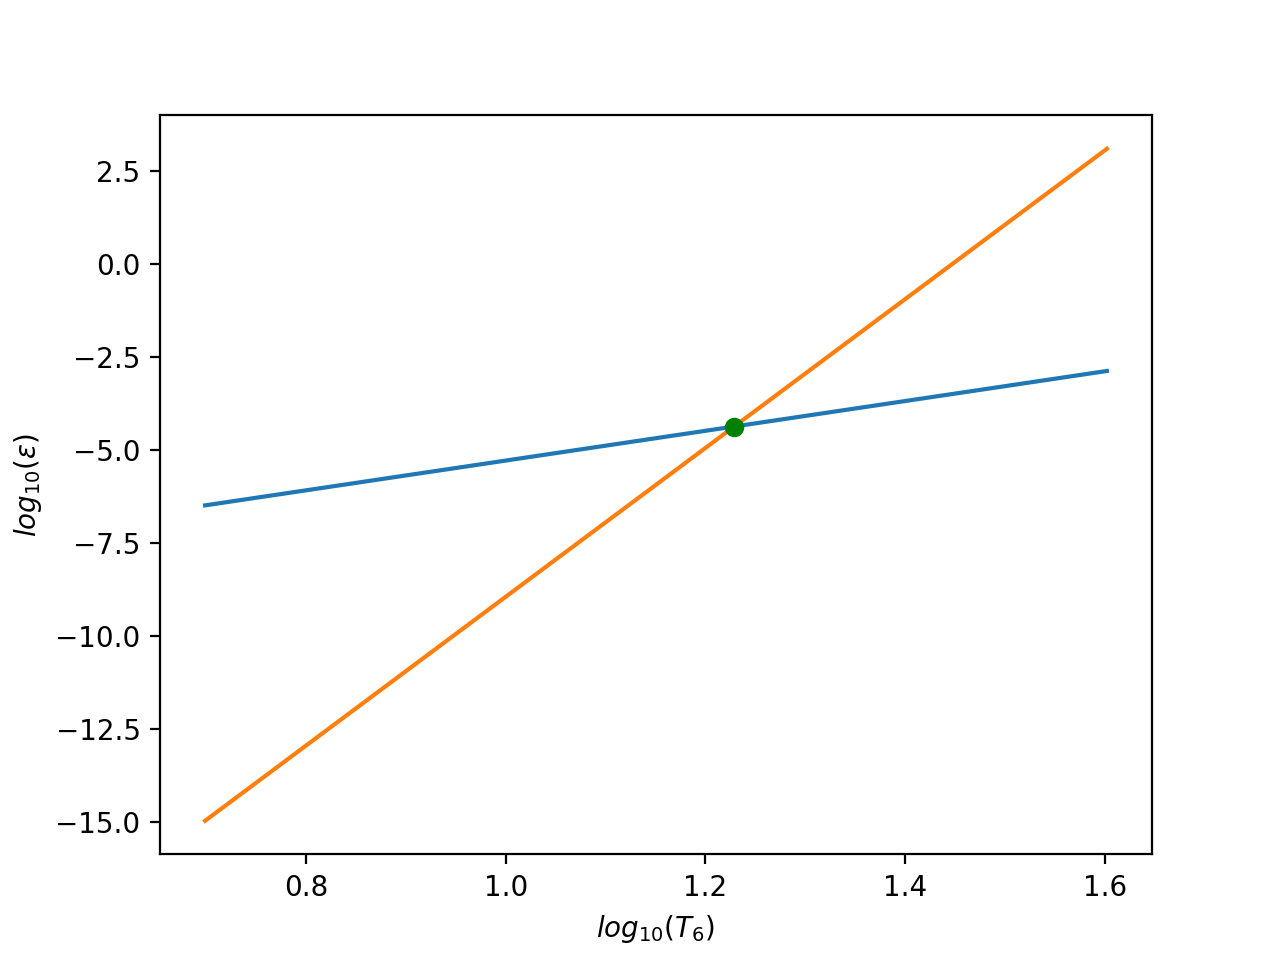
\includegraphics[width=7.5cm]{problem_3_fig_1.png} }}%
    \qquad
    {{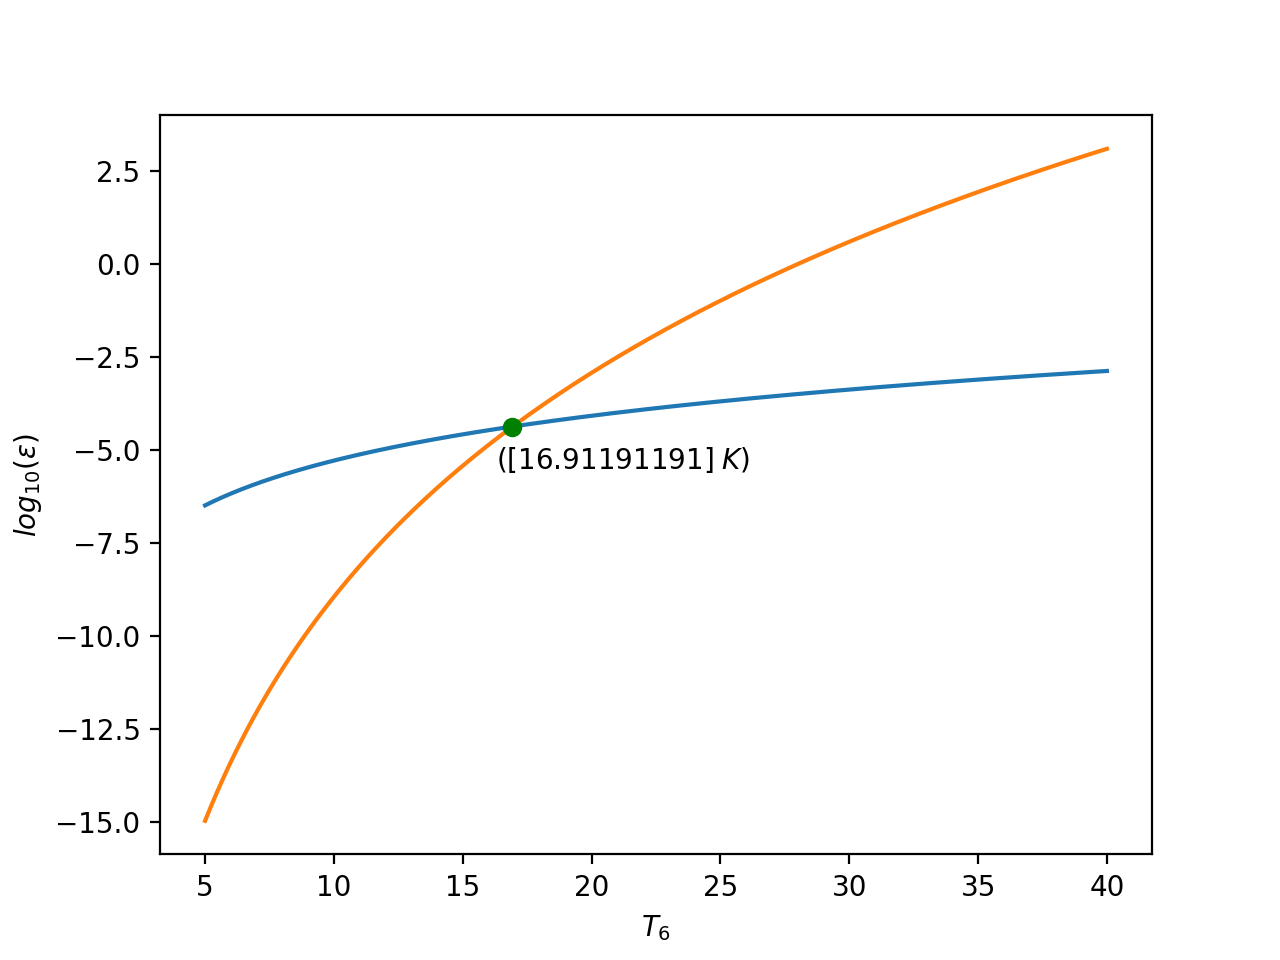
\includegraphics[width=7.5cm]{problem_3_fig_2.png} }}%
    \caption{The sub-figure on the left is the $log_{10} \epsilon \; \text{vs.} \; log_{10} T_{6}$. In order to figure out the temperature, the anti-log needs to be applied. The sub-figure on the right is the $log_{10} \epsilon \; \text{vs.} \; T_{6}$. When the two lines cross in this plot, it gives the temperature at which the PP chain and the CNO cycle will generate the same energy per unit time. Marked as a green dot and labeled in this figure is the point at which the two lines cross. The value of $T_{6}$ for this point on the figure is $16.9 \; K$. Which means that the plotted value and the calculated value in part (a) are in agreeance. }
    \label{fig:example}%
\end{figure}



\clearpage

\section*{Problem 4}

\subsubsection*{(a)}

The Hayashi forbidden region is shown below in the figure for 4 (b), this region is to the right of the linear line. The Hayashi forbidden region is the area in which it is impossible to construct stellar models in hydrostatic equilibrium. That is a star in this region would be unstable. A young star is able to be in this reagion, but once it has gone under convection, it will leave this zone. A star that is completely convection will be found on this Hayashi limit line.

\subsubsection*{(b)}

\begin{figure}[h!]
    \centering
    {{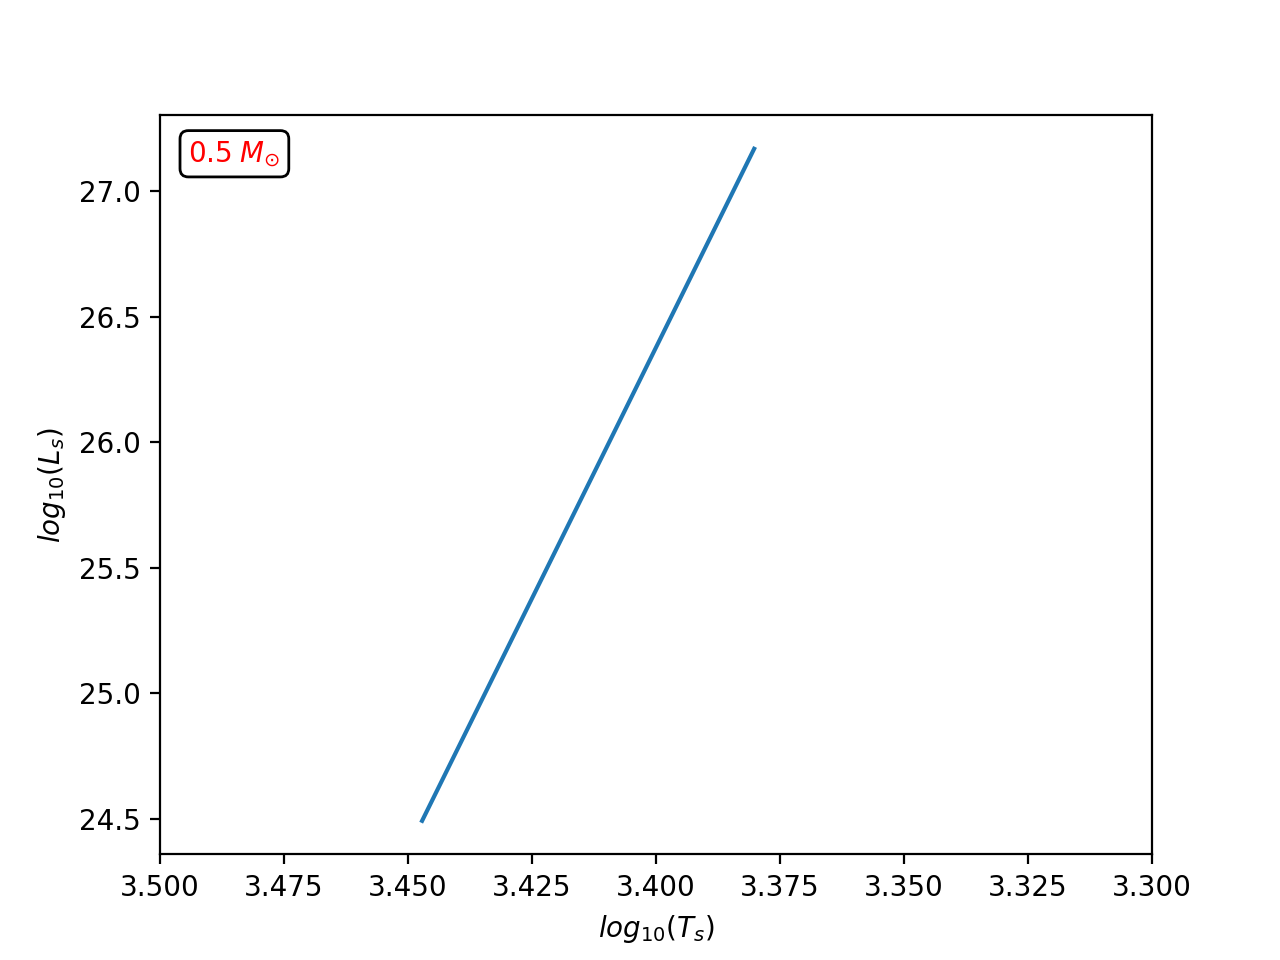
\includegraphics[width=15cm]{problem_4_fig_1.png} }}%
    \caption{This figure represents the \emph{Hayashi track} for a star with the mass of $M\textsubscript{\(\odot\)}$. Everything to the right of this linear line is considered the \emph{Hayashi forbidden region} described in part (a). }%
    \label{fig:example}%
\end{figure}

\clearpage

\section*{Appendix}

\subsection*{Python chart program}
\lstinputlisting{homework_4.py}

\clearpage


% -------------------------- EOD -------------------------- 
\end{document}